% questions.tex —— 1977 年·山东B卷 · 题目内容片段（无答案）
% 由 tools/generate_projects.py 依来源总账自 1977/1977_数学真题_山东B_试题.md 生成，勿手改（改源 MD 后重跑）


\gkpart{山东省(B)}

\begin{gktip}
\textbf{来源说明}：本题面依据固定源 PDF《1977山东B.pdf》第 1—7 页（书籍页码 57—63）逐题转录。源卷为题面与解答连续排印的扫描材料，每题题面下附「解：」或「证明：」，解答内容不转录进题面，留作解析正文的对照材料。原卷以「一、解下列各题」统领 6 个小题（原印作 1.至 6.），本库将这 6 个小题升为正式题号 1—6，原第二至六大题依次重排为第 7—11 题，题面内容未增删。原卷无分值标注，未见文理科说明。
\textbf{题号说明}：原卷大题号印作「一、」至「六、」，其中第一大题含 6 个小题（原印作 1.至 6.）；本库将小题 1—6 升为正式题号 1—6，原第二至六大题依次重排为第 7—11 题。卷末「参考题」两道沿用原卷序号「一、二」改作「参考题 1、参考题 2」，不计入正式题量。
\end{gktip}

\par\medskip

\begin{question}
\gkti{1}$\sqrt{(-a)^2}=?$

\end{question}
\begin{question}
\gkti{2}$\log_{\frac{1}{2}}\left[\left(1-\cos^2\dfrac{\pi}{6}\right)\operatorname{ctg}^{-2}\dfrac{\pi}{4}\right]=?$

\end{question}
\begin{question}
\gkti{3}写出下列函数的定义域：

（1） $y=\dfrac{\sqrt{|x-3|}}{x-2}$；

（2） $y=\lg(x+3)$.

\end{question}
\begin{question}
\gkti{4}写出过 $(0,\ 1)$ 和 $(2,\ 3)$ 两点的直线方程.

\end{question}
\begin{question}
\gkti{5}写出双曲线 $\dfrac{x^2}{16}-\dfrac{y^2}{9}=1$ 的渐近线方程.

\Needspace{0.4\textheight}
\end{question}
\begin{question}
\gkti{6}如图所示的二视图是什么几何体？
\nopagebreak[4]
\begin{center}% 1977 年山东B卷第 6 题：正四棱锥的二视图（按源卷第 2 页布局）
% 上：正面图（三角形，垂直点划中心线）；下：俯视图（正方形加两条对角线，十字中心线）
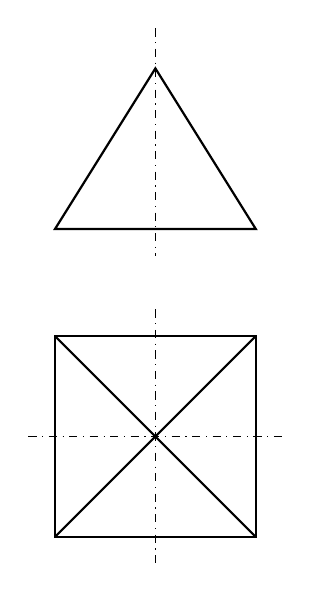
\begin{tikzpicture}[scale=0.85]
  % ---- 正面图：三角形 ----
  \coordinate (apex) at (0,2.4);
  \coordinate (bl) at (-1.5,0);
  \coordinate (br) at (1.5,0);
  \draw[thick] (bl)--(apex)--(br)--cycle;
  % 正面图垂直中心线（点划线，超出图形）
  \draw[dash dot] (0,3.0)--(0,-0.4);
  % ---- 俯视图：正方形 + 对角线 ----
  \coordinate (s1) at (-1.5,-1.6);
  \coordinate (s2) at (1.5,-1.6);
  \coordinate (s3) at (1.5,-4.6);
  \coordinate (s4) at (-1.5,-4.6);
  \draw[thick] (s1)--(s2)--(s3)--(s4)--cycle;
  \draw[thick] (s1)--(s3);
  \draw[thick] (s2)--(s4);
  % 俯视图十字中心线（点划线，超出图形）
  \draw[dash dot] (0,-1.2)--(0,-5.0);
  \draw[dash dot] (-1.9,-3.1)--(1.9,-3.1);
\end{tikzpicture}
\end{center}
\nopagebreak[4]
\Needspace{0.4\textheight}
\end{question}
\begin{question}
\gkti{7}$\square ABCD$ 的二邻边之比为 $1:2$，$M$ 为大边 $AB$ 的中点，连接 $MD$、$MC$，求证：$\angle DMC=\dfrac{\pi}{2}$.
\nopagebreak[4]
\begin{center}% 1977 年山东B卷第 7 题：平行四边形 ABCD，M 为大边 AB 的中点，连接 MD、MC（按源卷第 3 页布局）
% D 左上、C 右上、A 左下、M 在 AB 中点、B 右下
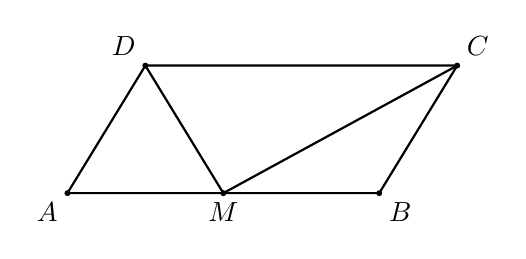
\begin{tikzpicture}[scale=0.9]
  \coordinate (A) at (0,0);
  \coordinate (M) at (2.2,0);
  \coordinate (B) at (4.4,0);
  \coordinate (D) at (1.1,1.8);
  \coordinate (C) at (5.5,1.8);
  \draw[thick] (A)--(B)--(C)--(D)--cycle;
  \draw[thick] (D)--(M);
  \draw[thick] (M)--(C);
  \fill (A) circle (1.2pt) node[below left] {$A$};
  \fill (M) circle (1.2pt) node[below] {$M$};
  \fill (B) circle (1.2pt) node[below right] {$B$};
  \fill (D) circle (1.2pt) node[above left] {$D$};
  \fill (C) circle (1.2pt) node[above right] {$C$};
\end{tikzpicture}
\end{center}
\nopagebreak[4]
\end{question}
\begin{question}
\gkti{8}

\nopagebreak[4]
\[
\frac{\sin\alpha}{2}\,x^2+x+\frac{1}{2\cos\alpha}=0
\qquad\left(0<\alpha<\frac{\pi}{2}\right)
\]

为关于 $x$ 的二次方程。当 $\alpha$ 为何值时，方程有两个不相等的实数根？它的根是什么？

\end{question}
\begin{question}
\gkti{9}试比较等底等高的正四棱锥和正圆锥的侧面积，看哪个的侧面积较小.

\Needspace{0.4\textheight}
\end{question}
\begin{question}
\gkti{10}一只船以 $v$ 海里/小时的速度向正北航行，在 $A$ 处望见灯塔在船的北 $\alpha$ 度东，继续航行 $t$ 小时后，在 $B$ 处望见 $S$ 在船的北 $\beta$ 度东，求第二次望见灯塔 $S$ 时船和灯塔的距离 $BS$.
\nopagebreak[4]
\begin{center}% 1977 年山东B卷第 10 题：船 A→B 向正北航行，灯塔 S 的方位角 α、β（按源卷第 5 页布局）
% A、B 在同一南北线上，S 在东北方向；β 标在 B 处，α 标在 A 处；右侧画北南西东方向标
\begin{tikzpicture}[scale=0.9,>=stealth]
  % 航线（南北线，虚线）
  \draw[dashed] (0,-0.5)--(0,4.9);
  \coordinate (A) at (0,0);
  \coordinate (B) at (0,3.2);
  \coordinate (S) at (1.9,4.3);
  \draw[thick] (A)--(S);
  \draw[thick] (B)--(S);
  \fill (S) circle (1.6pt);
  \node[above right] at (S) {$S$};
  \node[below left] at (A) {$A$};
  \node[left] at (B) {$B$};
  % A 处角 α（正北线与 AS 之间）
  \draw (0,0.75) arc[start angle=90,end angle=66,radius=0.75];
  \node at (0.30,0.92) {$\alpha$};
  % B 处角 β（正北线与 BS 之间）
  \draw (0,4.15) arc[start angle=90,end angle=30,radius=0.95];
  \node at (0.42,4.28) {$\beta$};
  % 方向标：北南西东
  \begin{scope}[shift={(2.9,1.5)}]
    \draw[->] (0,-0.9)--(0,0.9) node[above] {$\text{北}$};
    \node[below] at (0,-0.9) {$\text{南}$};
    \draw (-0.9,0)--(0.9,0);
    \draw[->] (0,0)--(0.9,0);
    \node[left] at (-0.9,0) {$\text{西}$};
    \node[right] at (0.9,0) {$\text{东}$};
  \end{scope}
\end{tikzpicture}
\end{center}
\nopagebreak[4]
\Needspace{0.4\textheight}
\end{question}
\begin{question}
\gkti{11}某隧道的横断面如图所示，已知隧道横断面的周长为 $23$ 米，试根据图所示尺寸，求当 $x$ 和 $y$ 为何值时，隧道的横断面的面积最大？最大面积是多少？（取 $\pi\approx 3$）（图尺寸单位：米）
\nopagebreak[4]
\begin{center}% 1977 年山东B卷第 11 题：隧道横断面（按源卷第 5 页布局）
% 上为半圆（半径 x，拱顶），下为矩形（高 y）；底部中央有宽 2x-1、高 0.5 的凸台阶，
% 台阶下基线画虚线；底部两段各标 0.5，台阶竖高标 0.5
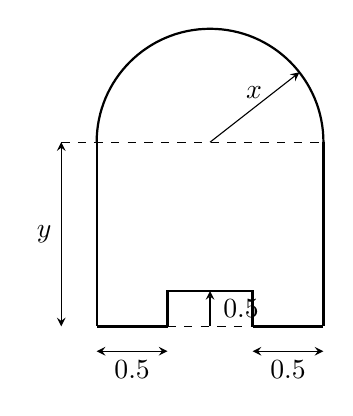
\begin{tikzpicture}[scale=0.9,>=stealth]
  % 半圆拱（圆心在拱弦线中点）
  \coordinate (L) at (-1.6,0);
  \coordinate (R) at (1.6,0);
  \draw[thick] (-1.6,0) arc[start angle=180,end angle=0,radius=1.6];
  % 拱弦线（虚线）
  \draw[dashed] (-2.1,0)--(1.6,0);
  % 半径 x 标注（箭头指向弧）
  \draw[->] (0,0)--(38:1.6);
  \node[above] at (0.62,0.48) {$x$};
  % 两侧竖墙
  \draw[thick] (-1.6,0)--(-1.6,-2.6);
  \draw[thick] (1.6,0)--(1.6,-2.6);
  % 底部：0.5 — 台阶（宽2x-1、高0.5）— 0.5
  \draw[thick] (-1.6,-2.6)--(-0.6,-2.6);
  \draw[thick] (-0.6,-2.6)--(-0.6,-2.1)--(0.6,-2.1)--(0.6,-2.6);
  \draw[thick] (0.6,-2.6)--(1.6,-2.6);
  % 台阶下基线（虚线）
  \draw[dashed] (-0.6,-2.6)--(0.6,-2.6);
  % 左侧高度 y 标注
  \draw[<->] (-2.1,0)--(-2.1,-2.6);
  \node[left] at (-2.1,-1.3) {$y$};
  % 底部左 0.5
  \draw[<->] (-1.6,-2.95)--(-0.6,-2.95);
  \node[below] at (-1.1,-2.95) {$0.5$};
  % 底部右 0.5
  \draw[<->] (0.6,-2.95)--(1.6,-2.95);
  \node[below] at (1.1,-2.95) {$0.5$};
  % 台阶高 0.5
  \draw[->] (0,-2.6)--(0,-2.1);
  \node[right] at (0.05,-2.35) {$0.5$};
\end{tikzpicture}
\end{center}
\nopagebreak[4]
\begin{gktip}
\textbf{参考题}
\end{gktip}

\Needspace{5\baselineskip}
\textbf{参考题 1．} 求极限：

\nopagebreak[4]
\[
\lim_{x\to0}\frac{\ln(1+x)}{x}.
\]

\textbf{参考题 2．} 用定积分求抛物线 $y^2=4x$ 与 $x^2=4y$ 所围成的曲边形面积.
\nopagebreak[4]
\begin{center}% 1977 年山东B卷参考题 2：抛物线 y²=4x 与 x²=4y 所围曲边形（按源卷第 6 页布局）
% 坐标轴标 X、Y，两抛物线按源卷记号标 X²=4Y（上）与 Y²=4X（右下），交点 (0,0) 与 (4,4)
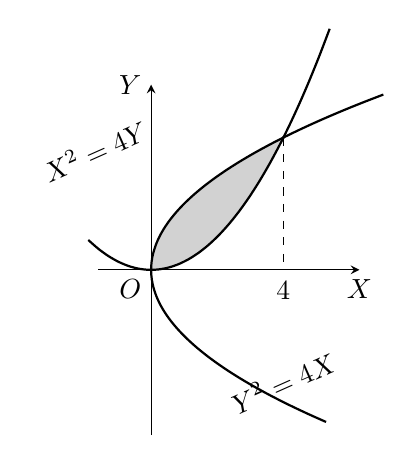
\begin{tikzpicture}[scale=0.42,>=stealth]
  % 坐标轴
  \draw[->] (-1.6,0)--(6.3,0) node[below] {$X$};
  \draw[->] (0,-5.0)--(0,5.6) node[left] {$Y$};
  \node[below left] at (0,0) {$O$};
  % 阴影区域：0≤x≤4 上 2√x 与 x²/4 之间
  \fill[gray!35]
    (0,0) plot[domain=0:4,smooth] (\x,{2*sqrt(\x)})
    -- plot[domain=4:0,smooth] (\x,{\x*\x/4}) -- cycle;
  % 抛物线 y²=4x（右开口，含左下延伸段）
  \draw[thick,domain=-4.6:5.3,smooth,samples=40] plot ({\x*\x/4},{\x});
  % 抛物线 x²=4y（上开口）
  \draw[thick,domain=-1.9:5.4,smooth] plot (\x,{\x*\x/4});
  % 交点 (4,4) 与虚线垂线
  \fill (4,4) circle (1.5pt);
  \draw[dashed] (4,4)--(4,0);
  \node[below] at (4,-0.05) {$4$};
  % 曲线标签（按源卷位置）
  \node[rotate=24] at (-1.7,3.6) {$X^2=4Y$};
  \node[rotate=24] at (4.0,-3.4) {$Y^2=4X$};
\end{tikzpicture}
\end{center}
\nopagebreak[4]

\end{question}